\section{Empirical Evaluation}
\label{sec:analysis}

In this section we evaluate the performance and scalability benefits
of the \iter keyword and its parallelization by providing empirical
results for two applications that originally included induction
variable state. We modified these applications to remove the explicit
induction variable state, and instead employ the \iter keyword. We
modified the StreamIt compiler as described in the last section.  The
experimental architecture is composed of 4 octal-core 2.00 GHz Intel
Xeon x7550 processors, each with 18 MB L3 caches. The architecture has
128 GB of available memory.

\subsection{MPEG-2 Motion Estimation}
\label{sec:mpeg}

\begin{figure}[t]
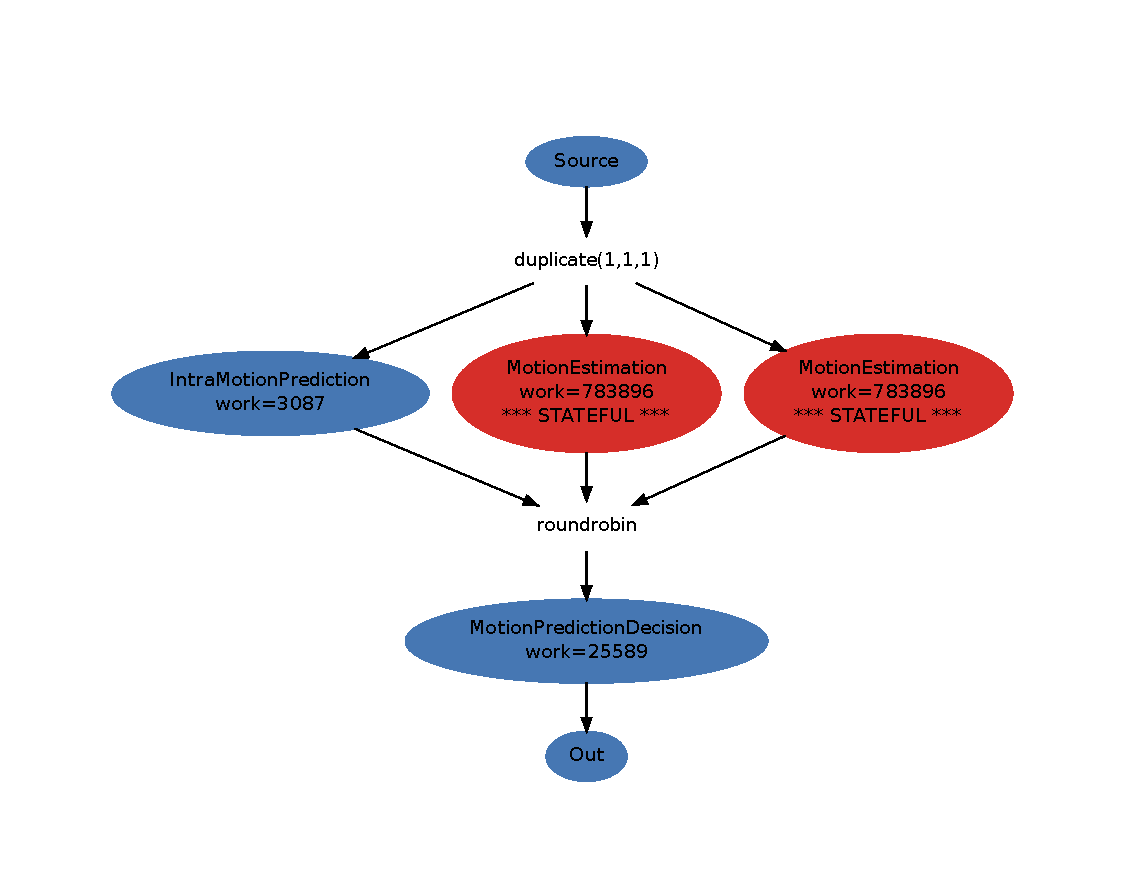
\includegraphics[width=3.3in]{figures/work_estimate_mpeg_motionestimation.pdf}
\caption{MPEG Motion Estimation stream graph.\protect\label{fig:mpegMEgraph}}
\end{figure}


This section presents an application of induction variables to the Motion Estimation compression subset of the MPEG-2 encoder.  MPEG-2 is a standard for coding moving pictures and audio information and has a wide variety of multimedia applications.  

The specification contains various types of compression, one of which is motion prediction.  Motion prediction takes advantage of the fact that frames of a video contain a large amount of duplicated scenes between consecutive frames.  Motion estimation attempts to generate predictions with respect to a set of reference frames obtained from previous or future pictures.  Accordingly, the MPEG-2 encoder can utilize forward and backward motion estimation to achieve this form of compression.  The process of Motion Estimation entails comparing pixel blocks between frames and forming a motion vector indicating a cartesian displacement of a macroblock between reference frames.  

The Motion estimation stream subgraph of the MPEG-2 encoder is illustrated in Figure~\ref{fig:mpegMEgraph}~\cite{drake-thesis}.  Each block of pixels will be tested against three types of prediction (no prediction, forward predicted, and backward predicted) to determine which is the best method for motion estimation.  The MotionEstimationDecision filter determines which is the best encoding technique for this macroblock.

The work estimation of this compression indicates the filter
MotionEstimation is stateful and contains the majority of the work.
The MotionEstimation filter pulls macroblocks at a time, iterating
through a two-dimensional array (16x16 macroblocks) along the picture.
The filter relies on induction variables to maintain its array
position.  We can apply the induction variable transformation on this
filter to remove the state in the filter.  Conversion to employ the
\iter keyword involved removing 11 lines and adding 2 lines.

Reference pictures are set using upstream messaging from later in the
stream graph. Currently the backend does not support the use of
upstream messaging, so for the purpose of benchmarking this
application, the reference picture is set to a dummy value and is
unchanged throughout the program. This does not detract from the data
parallelism introduced after removing the induction state. Upstream
messaging would simply require that sent messages be duplicated to all
fissed filters in the stream graph.

\begin{figure}[t]
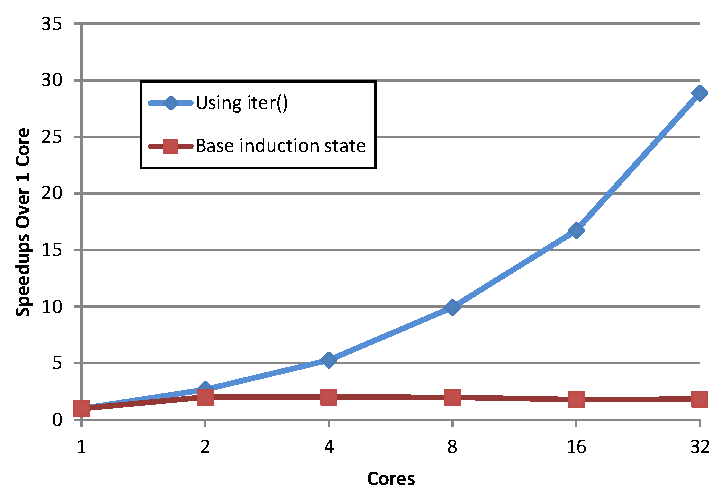
\includegraphics[width=3.3in]{figures/mpeg-results.pdf}
\caption{Speedups for MPEG-2 Encoder Motion Estimation subset, with and without induction variable state.  \protect\label{fig:mpeg-results}}
\end{figure}

Figure~\ref{fig:mpeg-results} shows the runtime figures for the
original stateful MPEG-2 motion estimation subset compared to the
stateless subset. There is a noticeable speedup for 2 cores for both
induction state and iteration keyword implementations. This can be
attributed to the stream graph, which is composed of two stateful
MotionEstimation filters. With 2 cores, these filters can be task
parallelized. The bottleneck in data parallelism is apparent as we
increase the number of cores past 2, as the majority of the work
cannot be partitioned and load-balanced effectively across multiple
cores.

We can see significant improvements to runtime after making this
subset stateless and exposing data parallelism. There is a 4.93X
speedup on 8 cores, 9.30X speedup on 16 cores, and 15.62X speedup on
32 cores between the base induction variable and iteration keyword
implementations.

\subsection{FIRBank}
\begin{figure}[t]
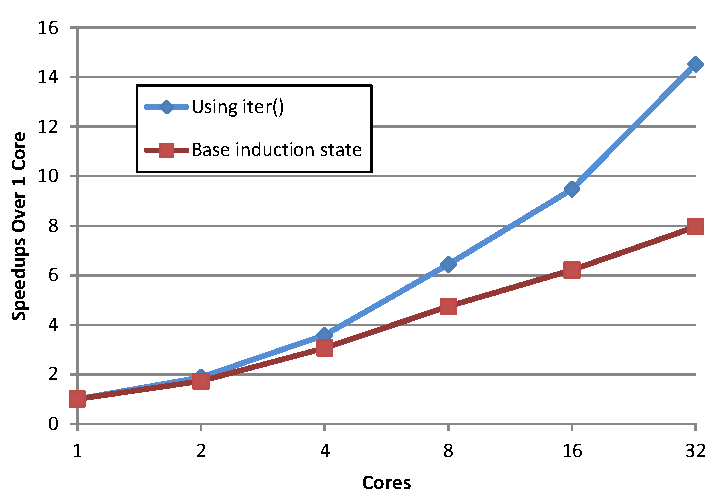
\includegraphics[width=3.3in]{figures/firbank-results.pdf}
\caption{Speedups for FIRBank, with and without induction variable state.  \protect\label{fig:firbank-results}}
\end{figure}

The FIRBank benchmark contains multiple finite impulse response
filters each with a different impulse response coefficient array. This
benchmark is used in speech processing applications. FIRBank contains
one filter that uses induction variable state with 3.94\% of program's
work. This filter, Multiply, maintains induction state in an index
that traces through the rows of a two dimensional array. Each
invocation performs complex multiplication on the stream input values
and the array elements of that specified row.  The conversion to the
\iter keyword version removed 5 lines and added 1 line.

The original version with explicit state is partitioned into a 3
filter pipeline: stateless filter, stateful filter (with explicit
induction state), and a stateless filter. The stateless filters are
data-parallelized, but the first requires data to be collected in a
joiner (in a synchronization point) before passing on to the
unparallelized stateful filter. Furthermore, output from the stateful
filter must be communicated to all cores of the chip as the last
stateless filter has fission products on all cores.  In the \iter
version, the entire application is fused to a single filter that can
be data parallelized.  There is no inter-core communication in the
fused and parallelized final version.

Figure~\ref{fig:firbank-results} indicates the speedups over 1 core
for both induction state and iteration keyword implementations.
Between the two implementations, there is 1.36X speedup on 8 cores,
1.58X speedup on 16 cores, and 1.83X speedup on 32 cores for the
iteration keyword implementation. This abides fairly closely with the
model as described in Section ~\ref{sec:model-analysis}.
